\documentclass{beamer}

\title{Medieval Madness pinball: Battle for the Kingdom}
\author{Frostsnow}
\date{April 12th, 2025}

\usetheme[hideothersubsections]{Hannover}
\usecolortheme{sidebartab}

\begin{document}

\begin{frame}
  \titlepage
\end{frame}

\begin{frame}
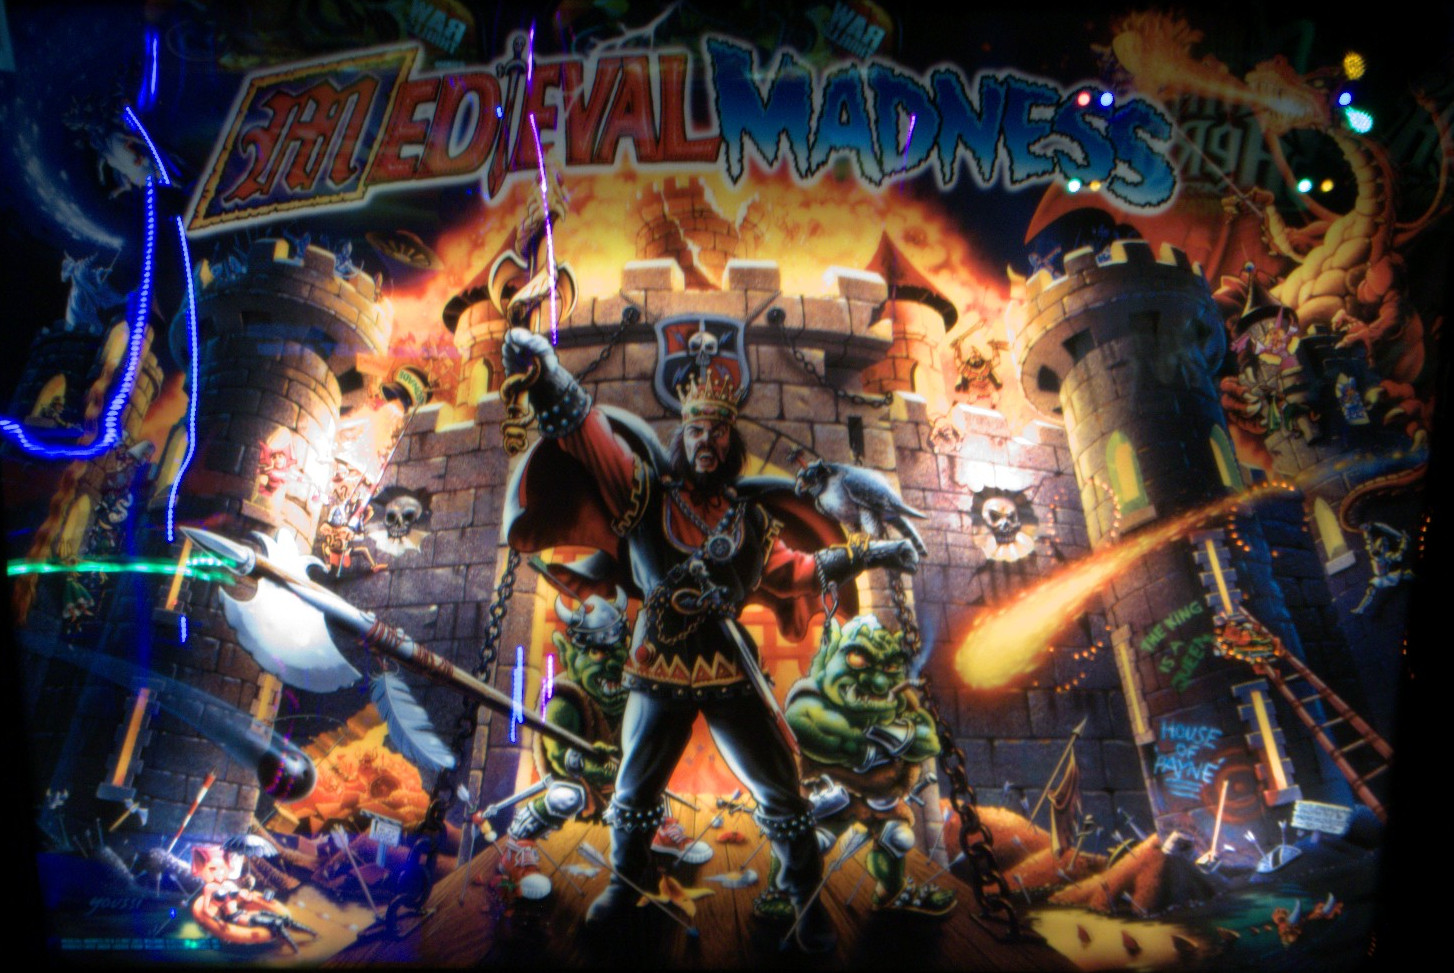
\includegraphics[width=\textwidth]{topper.jpg}
\end{frame}

\section{Overview}
\begin{frame}{Shots}
\begin{columns}
\begin{column}{0.5\textwidth}
	\begin{itemize}
		\item Castle
		\item Lock
		\item Merlin's Magic (``eject'' or ``right eject'')
		\item Peasant
		\item Damsel
		\item Joust
		\item Catapult
		\item Trolls
	\end{itemize}
\end{column}
\begin{column}{0.5\textwidth}
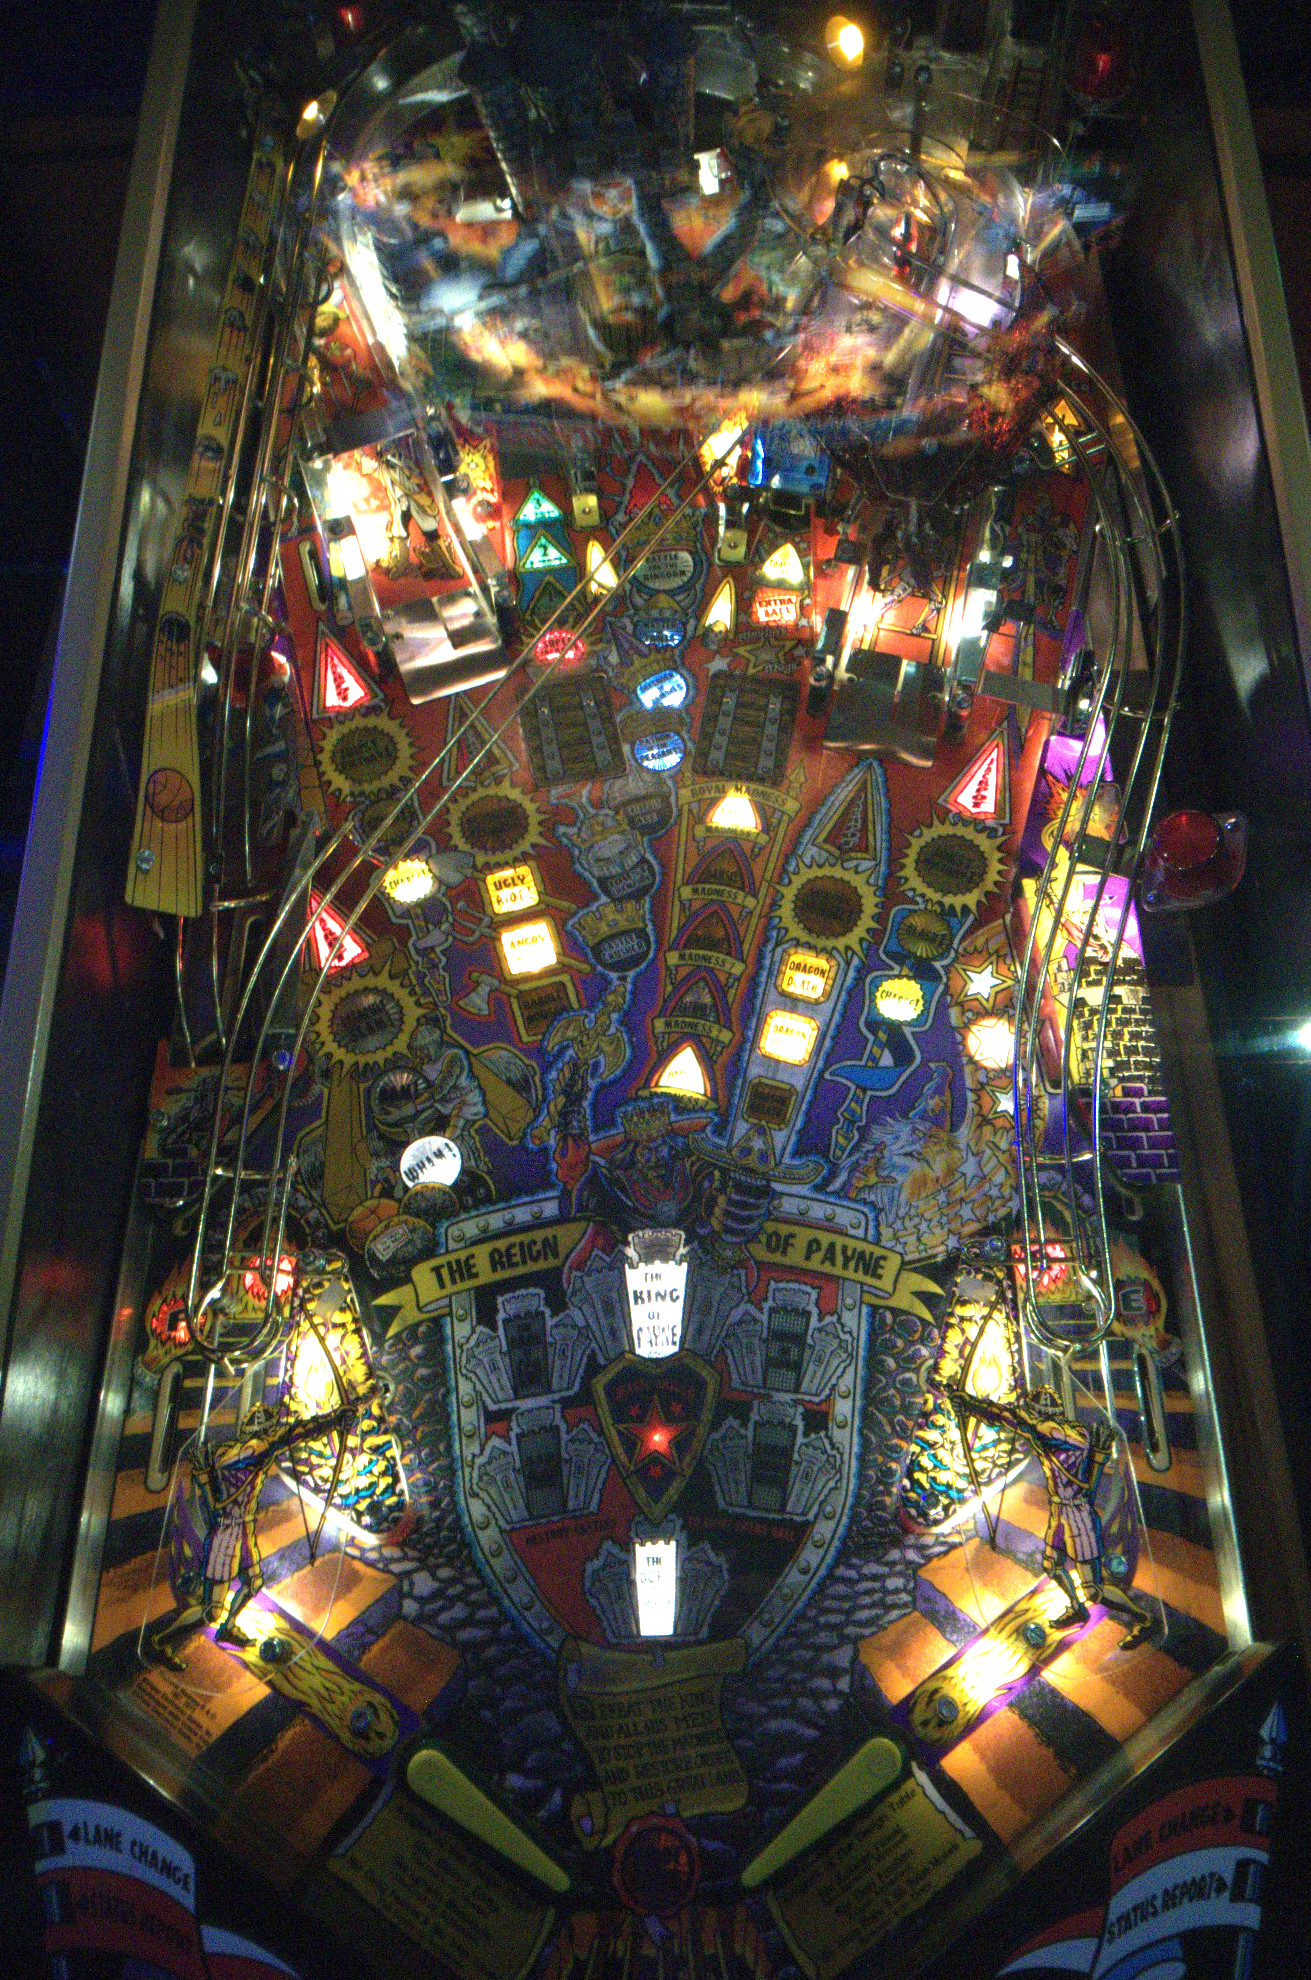
\includegraphics[width=\textwidth]{playfield.jpg}
\end{column}
\end{columns}
\end{frame}

\begin{frame}{``Features''}
\begin{itemize}
	\item Castle Multiball
	\item Multiball Madness
	\item Royal Madness
	\item Hurry ups
	\item Save the Children!
	\item Barnyard Multiball
\end{itemize}
\end{frame}

\begin{frame}{``Tiers''}
\begin{itemize}
	\item Emphasis: extend game time
	\item[]
	\item Tier 1: Extra ball
	\item Tier 2: Replay
	\item Tier 3: Royal Madness
	\item Tier 4: Battle for the Kingdom
\end{itemize}
\end{frame}

\section{Gameplay}

\begin{frame}{Beginning: Skill Shot\ldots}
\begin{columns}
\begin{column}{0.5\textwidth}
	\begin{itemize}
		\item Two lights in the corner
		\item Use flippers to rotate light
		\item Ensure ball moves over the lit lane
		\item Basically impossible to miss
		\item 5x bonus multiplier, 50,000+ points
	\end{itemize}
\end{column}
\begin{column}{0.5\textwidth}
	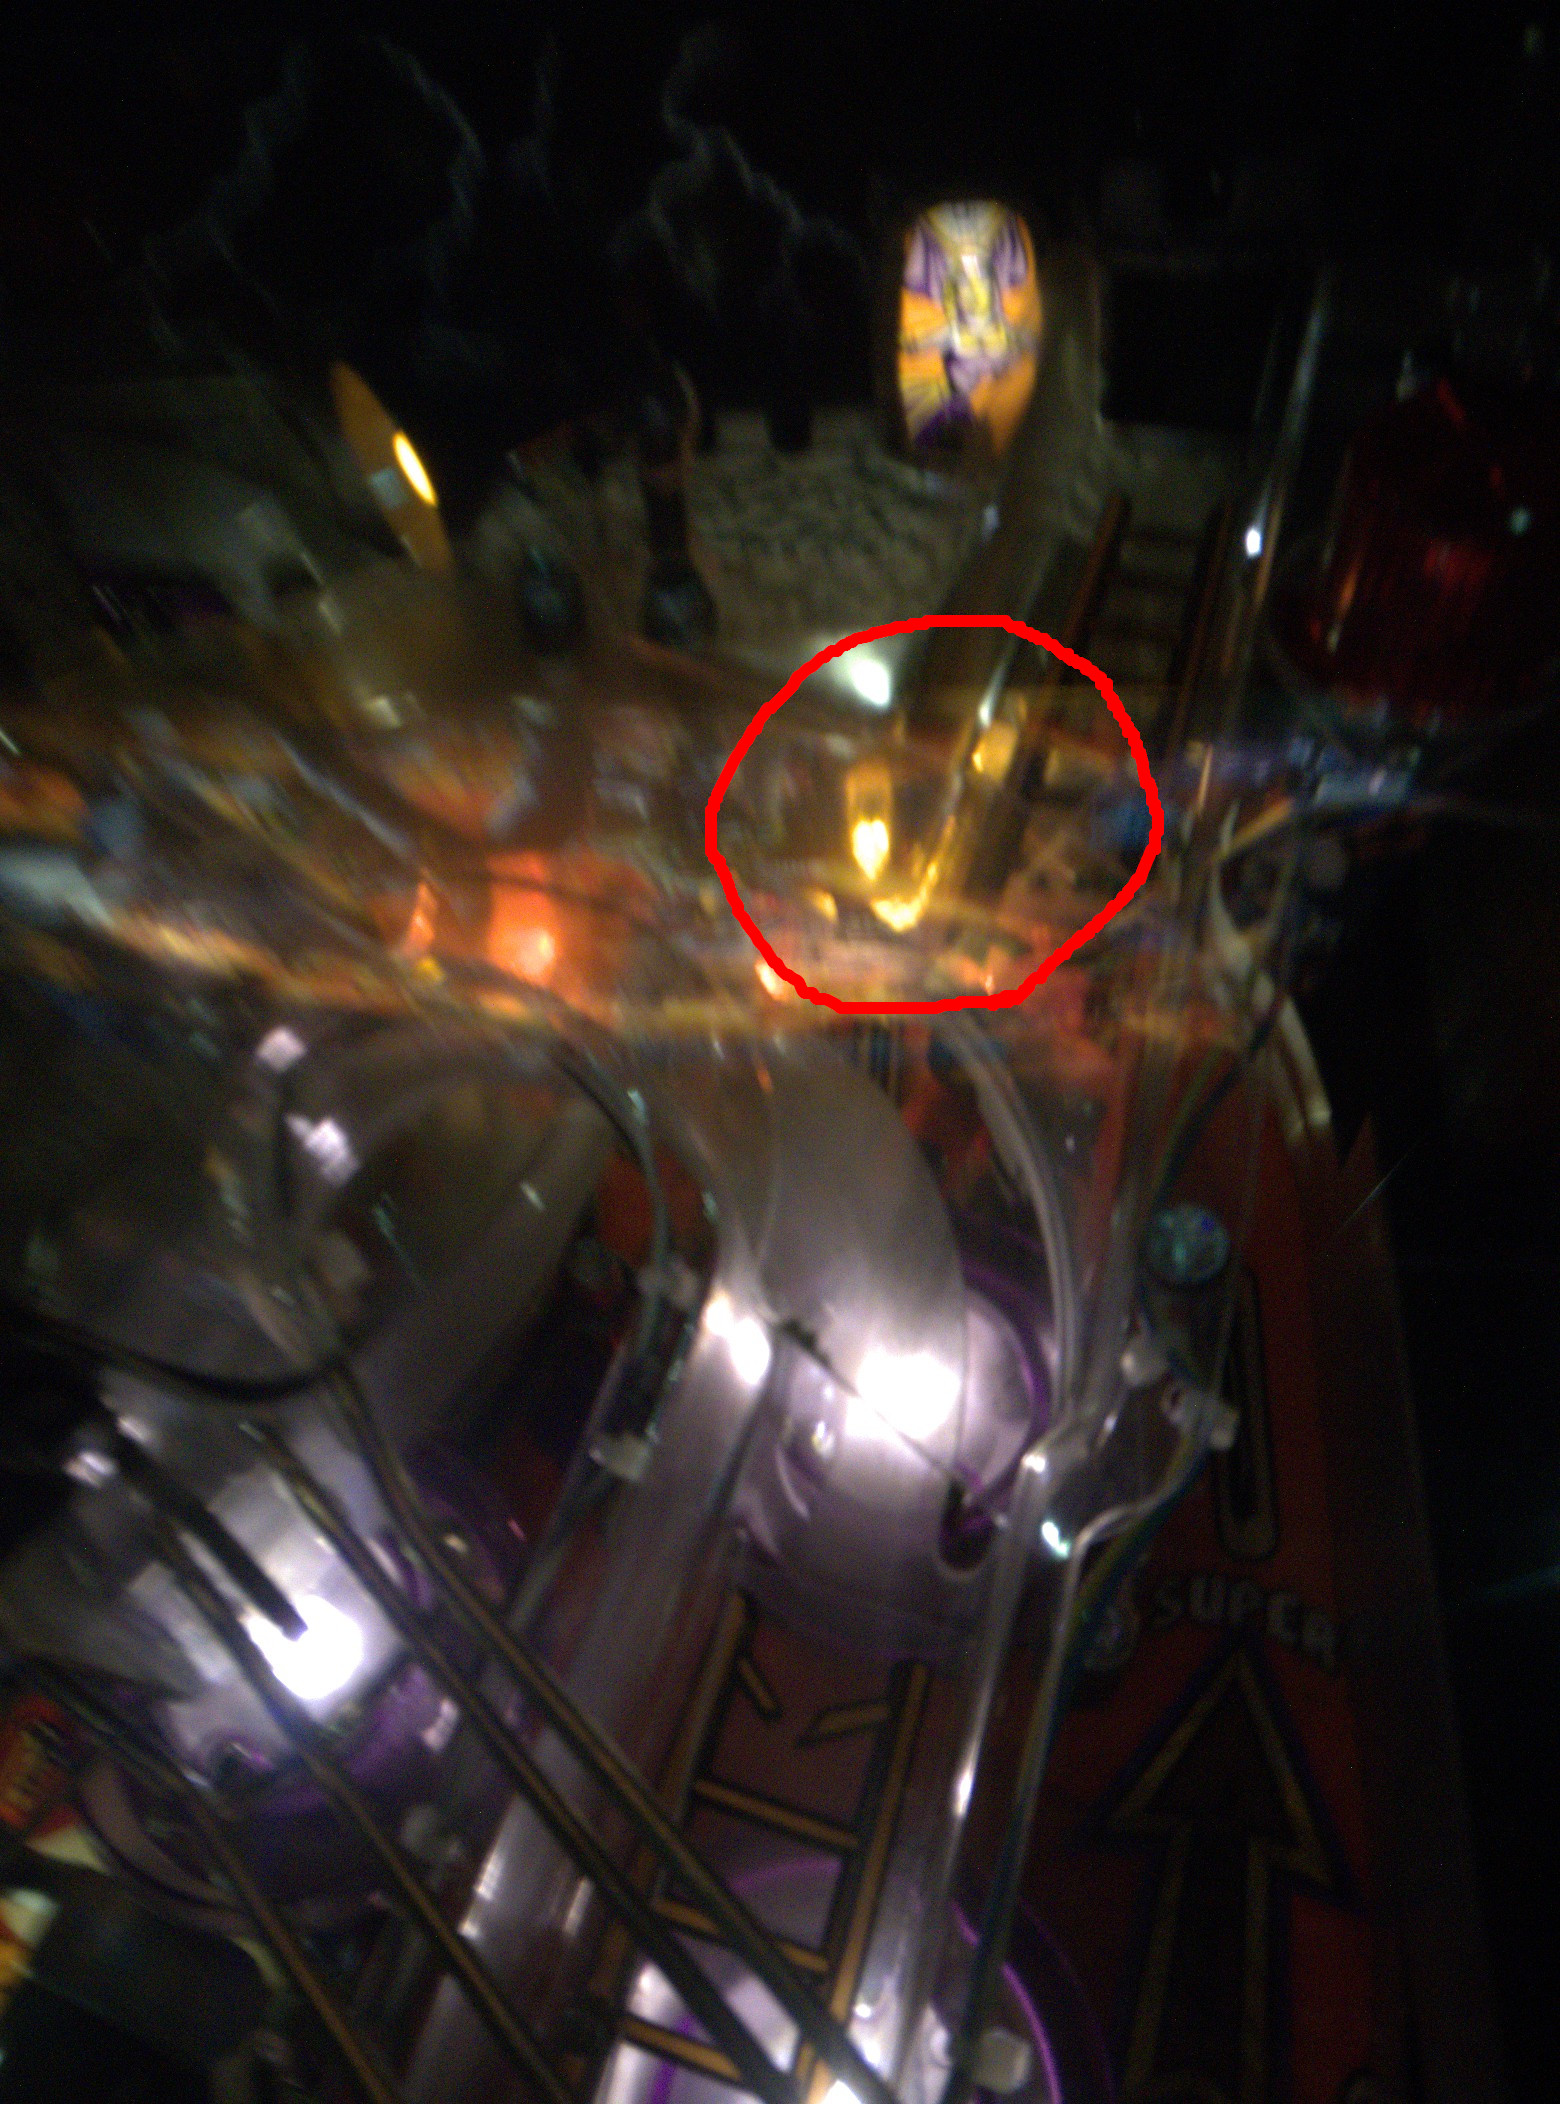
\includegraphics[width=\textwidth]{skill_shot.jpg}
\end{column}
\end{columns}
\end{frame}

\begin{frame}{Beginning (cont.): \ldots or Super Skill Shot?}
\begin{itemize}
	\item Hold left flipper during launch
	\item Ball shoots out of left orbit
	\item Three steps:
	\begin{itemize}
		\item Get control (or get lucky)
		\item Make one of the lane shots (100,000)
		\item Complete hurry up (shoot the castle) (1,000,000 max)
	\end{itemize}
	\item Getting control is really hard
	\begin{itemize}
		\item Dropping flipper always drains for me
		\item Do nothing or flip based on ball trajectory
		\item Left-ish: do nothing, ball bounces from left to right and back, make damsel shot
		\item Right-ish: Flip and pray
		\item Look for the rightward hook
	\end{itemize}
\end{itemize}
\end{frame}

\begin{frame}{Feature: Castles}
\begin{columns}
\begin{column}{0.5\textwidth}
\begin{itemize}
	\item Three states
	\begin{itemize}
		\item Drawbridge up
		\item Gate closed
		\item Open
	\end{itemize}
\end{itemize}
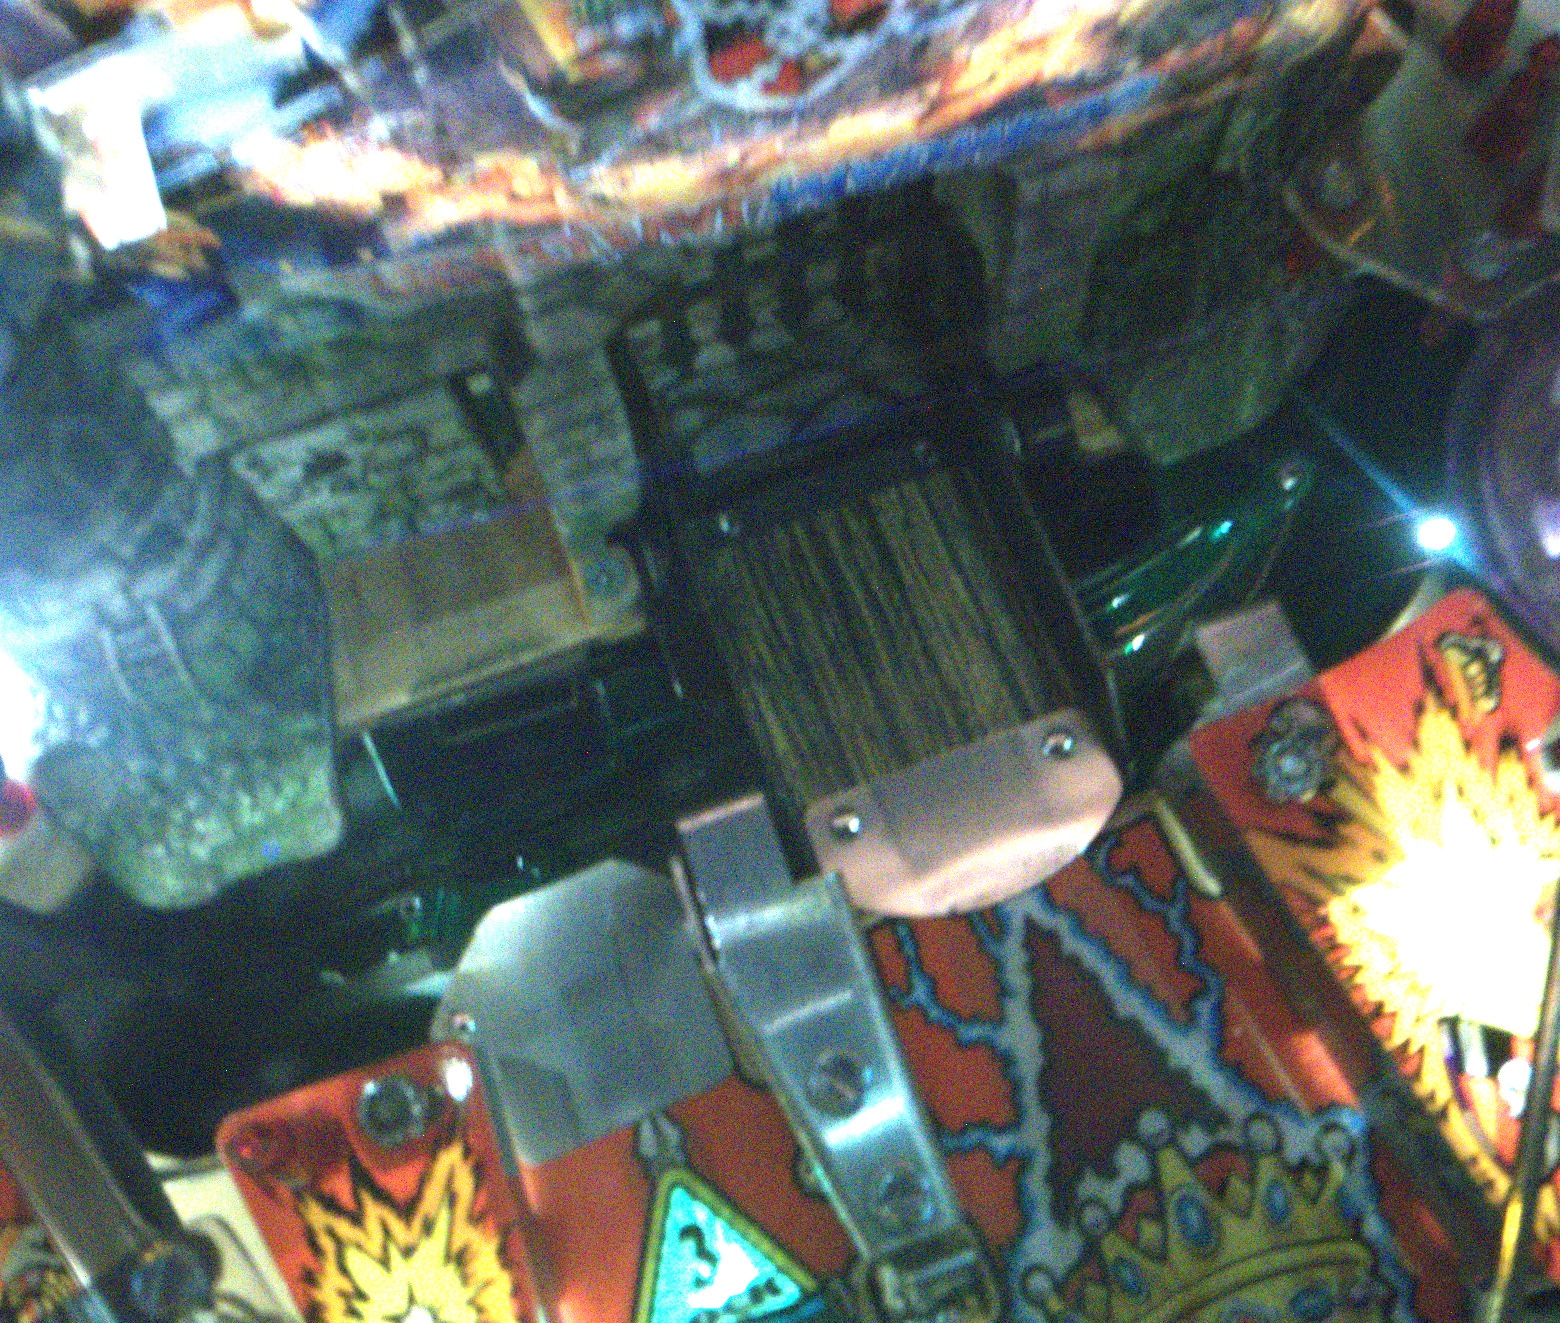
\includegraphics[width=\textwidth]{castle_gate.jpg}
\end{column}
\begin{column}{0.5\textwidth}
	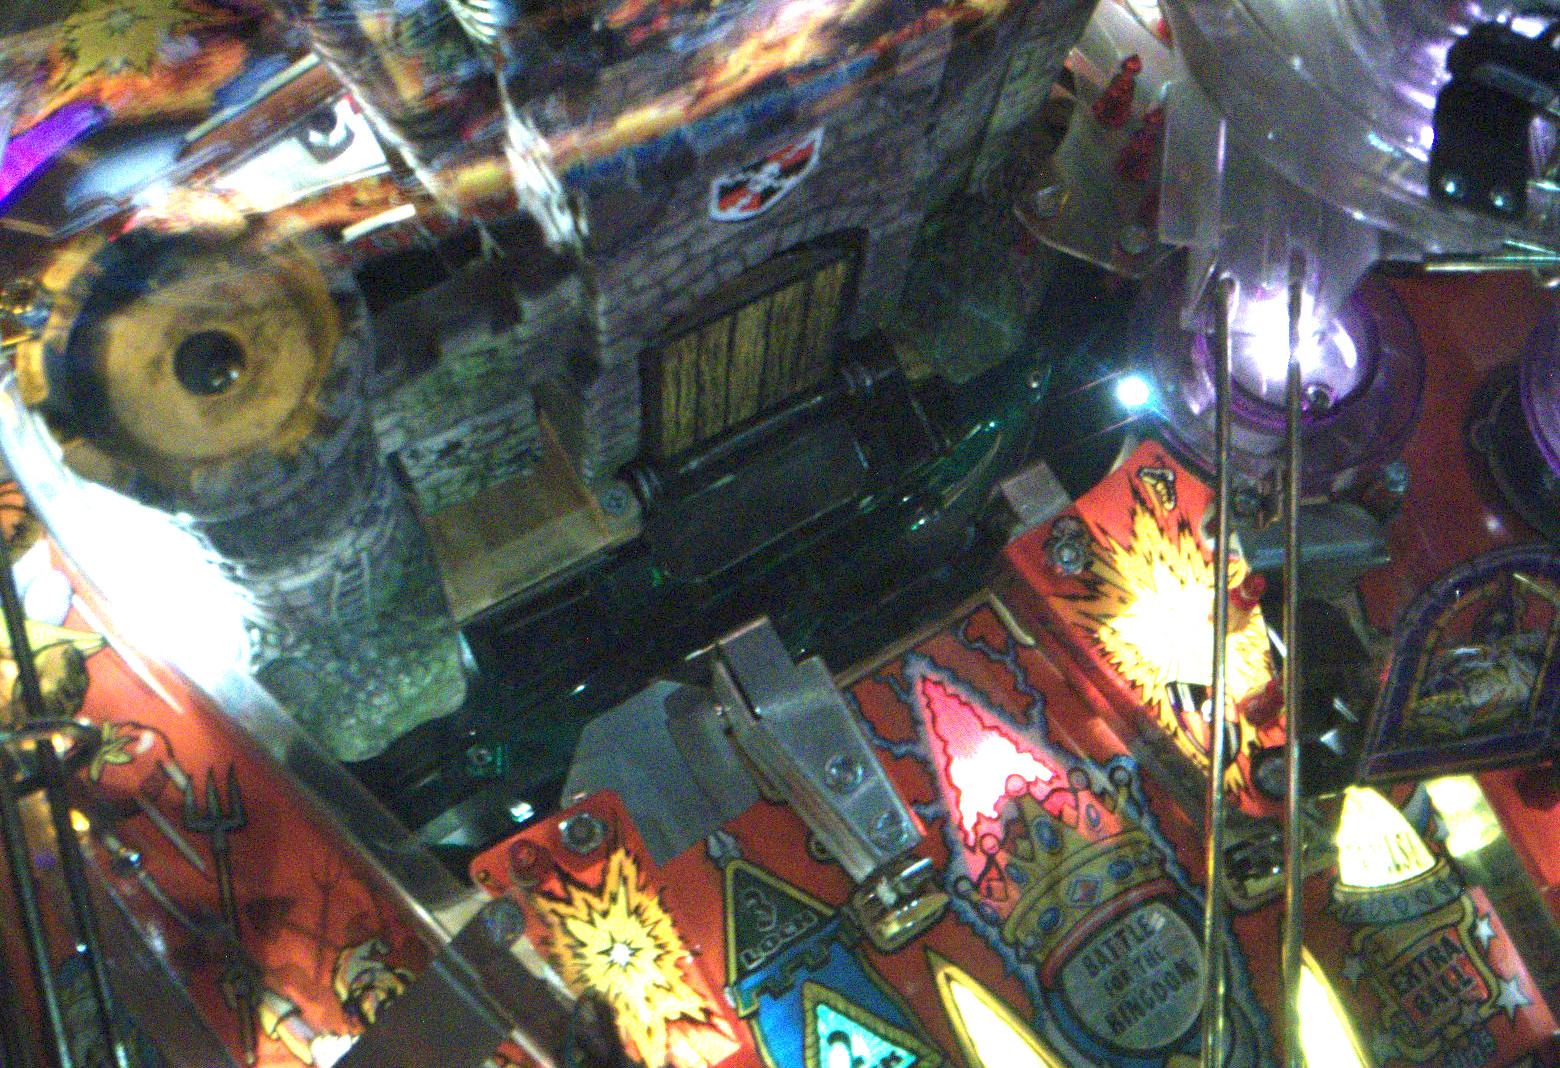
\includegraphics[width=\textwidth]{castle_up.jpg}
	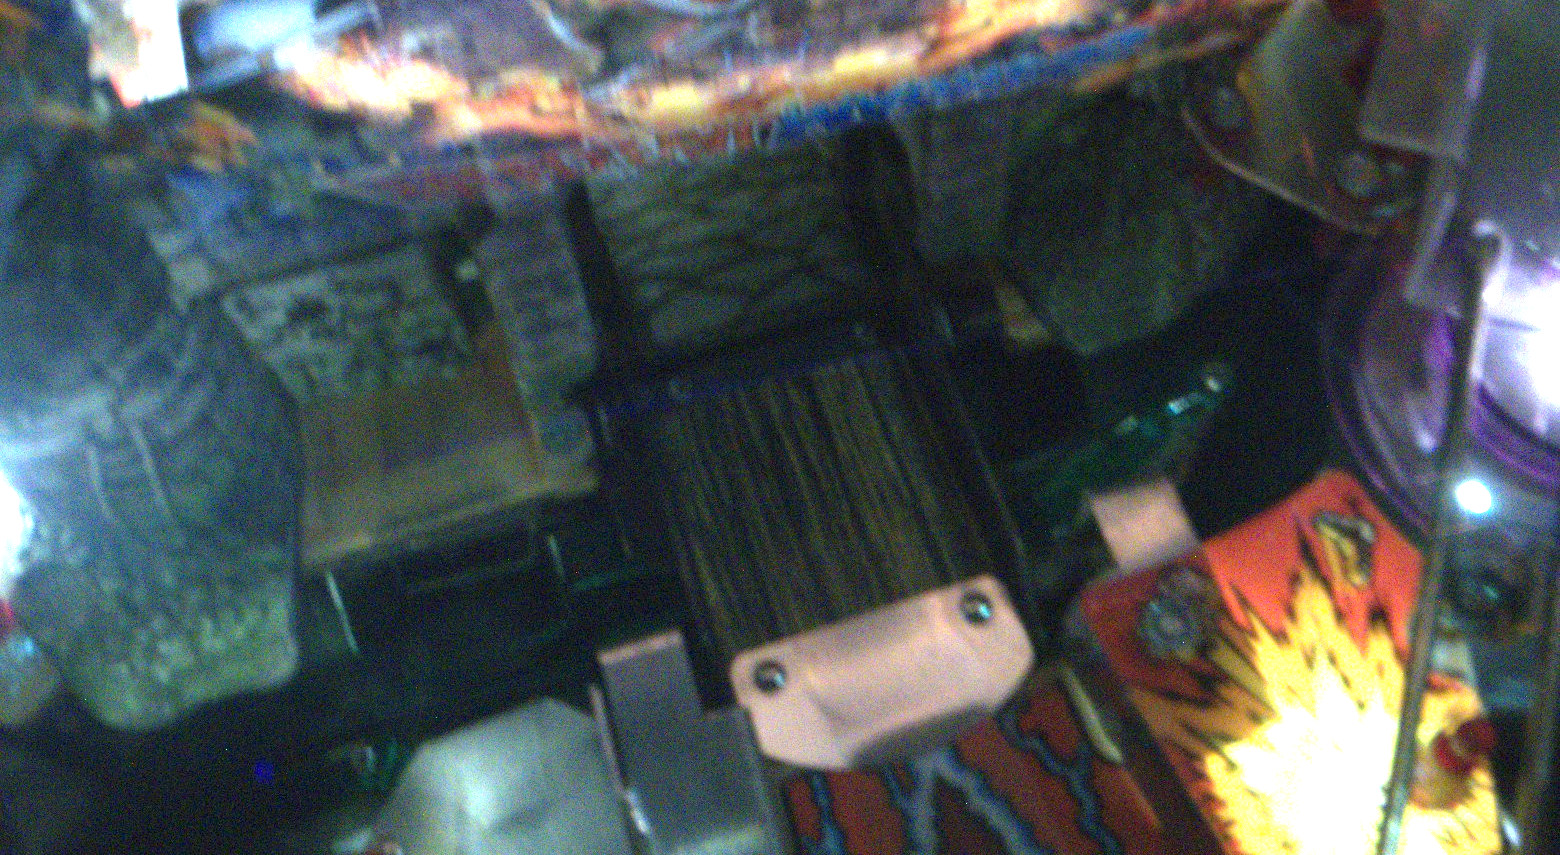
\includegraphics[width=\textwidth]{castle_open.jpg}
\end{column}
\end{columns}
\end{frame}

\begin{frame}{Feature: Castles (cont.)}
\begin{itemize}
	\item Shoot drawbridge once to lower
	\item Shoot gate twice (200,000) to open
	\item Shoot into castle to destroy (2,000,000)
	\item Six castles to destroy
	\begin{itemize}
		\item Drawbridge \& gate shots each increase by one along with multiplier
		\item Payne is special: 1,000,000 for gate, 20,000,000 for castle
	\end{itemize}
	\item Drawbridge is safe, but no points
	\item Gate is dangerous, gives points
	\item Shoot with power, watch closely, be prepared to nudge the table
\end{itemize}
\end{frame}

% TODO: It'd be good to show Merlin's Magic hole w/ Extra Ball lit here
\begin{frame}{Tier 1: Extra ball}
\begin{itemize}
	\item Shoot the castle!
	\item Destroy 2 castles to light Extra Ball
	\item Shoot Merlin's Magic to claim
	\item []
	\item Flip near base of the flipper
	\item Left flipper, drawbridge, left flipper loop
	\item Disregard trolls, shoot castle
	\item Avoid Merlin's Magic unless drawbridge is down
	\item Beware gate from right flipper
	\begin{itemize}
		\item Maybe lock shot instead
	\end{itemize}
\end{itemize}
\end{frame}

\begin{frame}{Feature: Castle Multiball}
\begin{columns}
\begin{column}{0.75\textwidth}
\begin{itemize}
	\item Not needed for Battle of the Kingdom
	\item \ldots still very useful
	\item Lock shot: 3 times first, 6 times subsequent
	\begin{itemize}
		\item Get at least once
	\end{itemize}
	\item 3 ball multiball, 3 stages:
	\begin{itemize}
		\item 5 jackpot shots (750,000): peasant or damsel ramps
		\item Lock shot for super jackpot (1,500,000), light Extra Ball
		\item All lanes super jackpots (1,500,000)
	\end{itemize}
	\item Castles still active
	\item Tier 1?  Shoot castles
	\item Tier 2 or 3? Go for jackpots then lock shot for Extra Ball
\end{itemize}
\end{column}
\begin{column}{0.25\textwidth}
	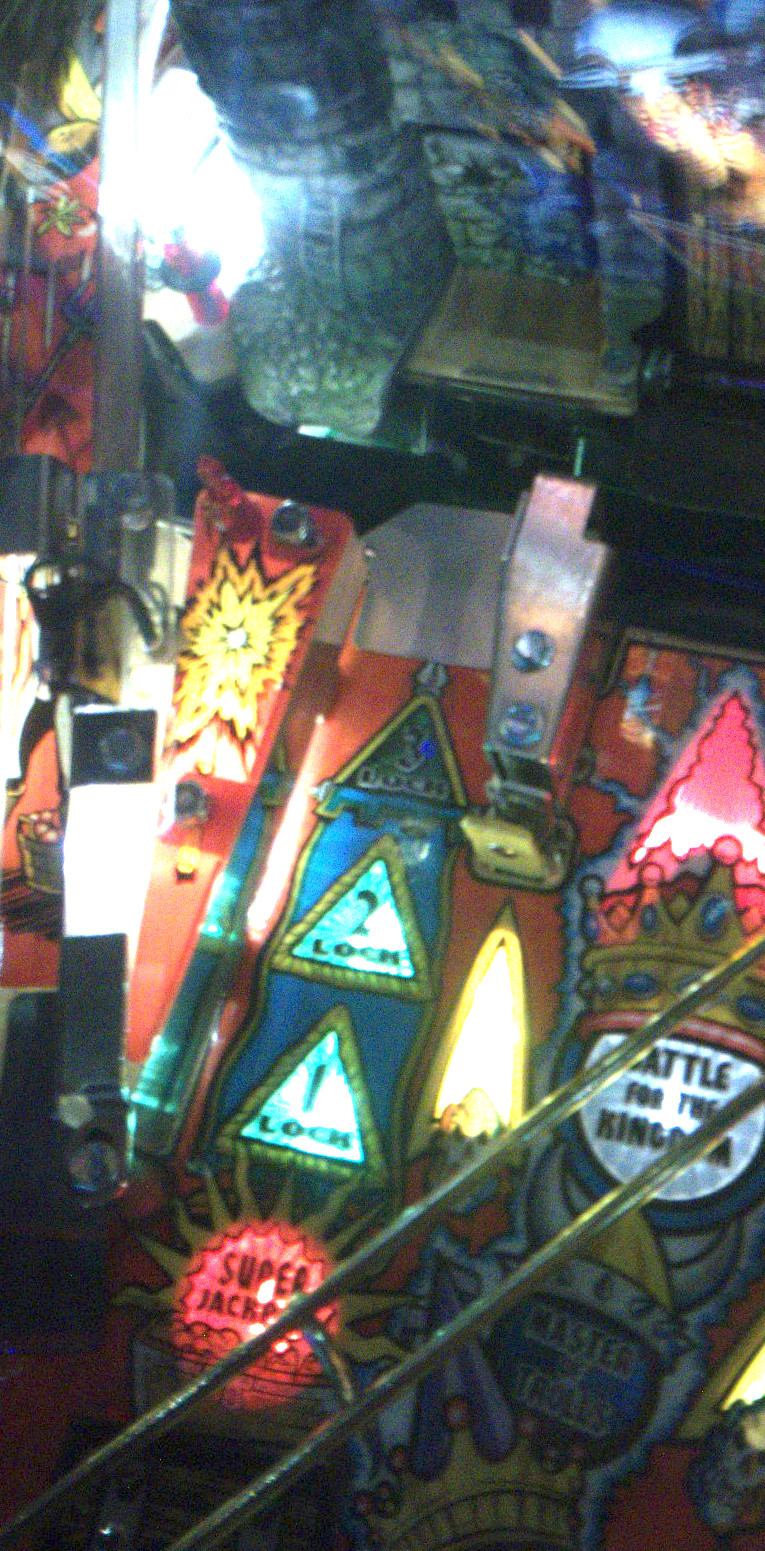
\includegraphics[width=\textwidth]{lock_shot.jpg}
\end{column}
\end{columns}
\end{frame}

% TODO: Picture of being knighted (replay)
\begin{frame}{Tier 2: Replay}
\begin{itemize}
	\item Get a ton of points!  \textbf{POP!}
	\item Base value varies: 15,000,000 - 30,000,000 observed
	\begin{itemize}
		\item Value increases by 50\% of base value when chained
	\end{itemize}
	\item Strategy depends on value, skill, and inclination
	\item Low value: ($\leq 21,000,000$)
	\begin{itemize}
		\item Destroy the third castle!
		\item \ldots that usually does it
	\end{itemize}
	\item Larger values
	\begin{itemize}
		\item 4 castles is not easy\ldots and rather repetetive
		\item Need a good multiball
		\item Lock shot, damsel, and peasants
		\item Two madnesses \& trolls a great start
		\item Wait, whatnesses?!  (see next slide!)
	\end{itemize}
\end{itemize}
\end{frame}

\begin{frame}{Feature: Multiball Madness}
\begin{columns}
\begin{column}{0.8\textwidth}
\begin{itemize}
	\item 5 ``madness'' lights
	\item Complete lane or trolls to light corresponding madness
	\item More madnesses: more balls, bigger jackpots
	\begin{itemize}
		\item 1 madness: 2 balls
		\item 2-4 madnesses: 3 balls
		\item 5 madnesses: 4 balls
	\end{itemize}
	\item Activate via eject shot
	\begin{itemize}
		\item All lanes jackpots
		\item Madness lanes super jackpots
		\item Lock shot double super jackpot
		\item Troll madness: Left troll, shoot for jackpot, other troll pops up, repeat
		\begin{itemize}
			\item 10 troll kills for Master of Trolls
			\item Each hit counts as a kill (instead of 3)
			\item Tip: shoot trolls until Master of Trolls lit
		\end{itemize}
	\end{itemize}
\end{itemize}
\end{column}
\begin{column}{0.2\textwidth}
	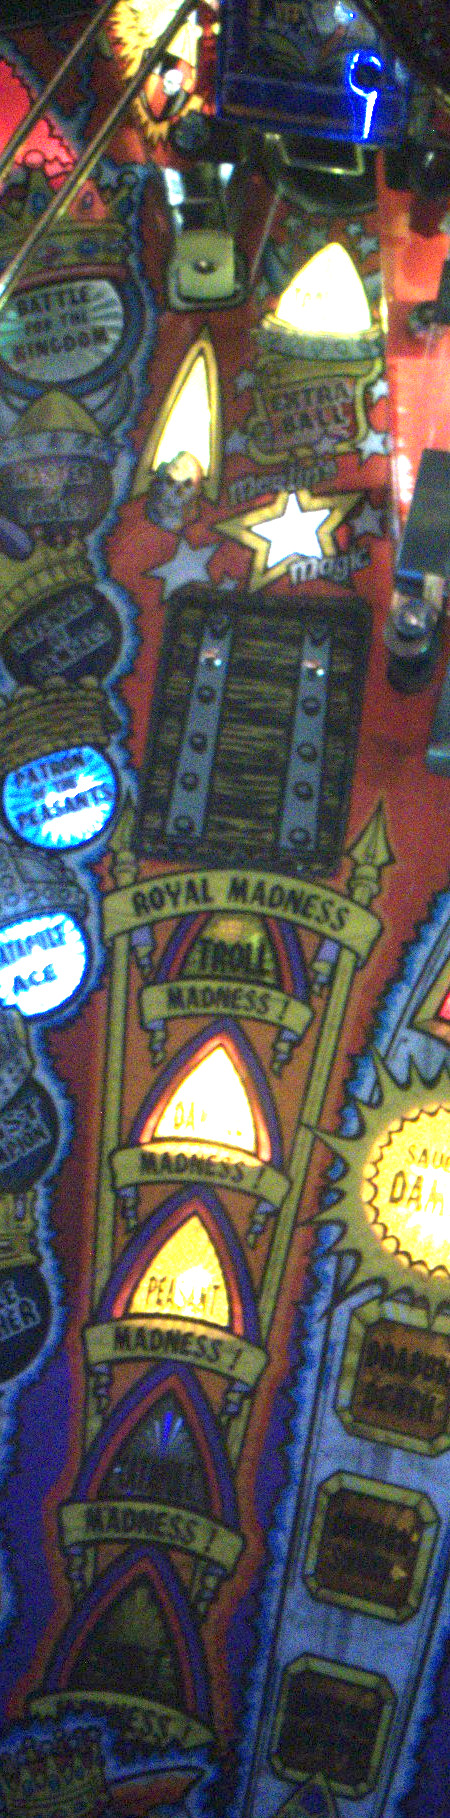
\includegraphics[width=\textwidth]{royal_madness.jpg}
\end{column}
\end{columns}
\end{frame}

\begin{frame}{Feature: Multiball Madness (cont.)}
\begin{itemize}
	\item Eject shot can also start trolls
	\begin{itemize}
		\item This is a Good Thing
		\item Trolls are hard to kill, easier with more balls
		\item Finishing trolls during madness \emph{adds} troll madness, restores drained balls, re-activates ball save
		\item Advice: always stack trolls with multiball madness
	\end{itemize}
	\item Castles still active
	\item Must activate Royal Madness before next multiball madness
	\item If multiball madness done, hurry up activated instead
\end{itemize}
\end{frame}

\begin{frame}{Feature: Multiball Madness (cont.)}
\begin{itemize}
	\item To madness or not to madness?
	\begin{itemize}
		\item 5 madnesses lit: Obviously
		\item Start Trolls lit, 4 madnesses lit: Obviously
		\item Start Trolls lit, 2 madnesses lit: Good
		\item Start Trolls lit, 1 madness lit: Meh
		\item 2 madnesses (not troll) lit: Meh
		\item 1 madness lit: Desperation move to shoot castles
	\end{itemize}
\end{itemize}
\end{frame}

% TODO: Picture of all madnesses lit.
\begin{frame}{Tier 3: Royal Madness}
\begin{itemize}
	\item Finish multiball madness, light all madnesses, eject shot to activate
	\item Note: \emph{activation} counts as tier 3, not completion!
	\item Master damsel and peasant shots first
	\begin{itemize}
		\item Loop between damsel and peasant ramps
		\item Useful for castle multiball
		\item \ldots and activating madnesses
	\end{itemize}
	\item Joust shot next
	\begin{itemize}
		\item Lanes are linked
		\item \ldots but not in Battle for the Kingdom
		\item Good to master both
	\end{itemize}
	\item Catapult shot last
	\begin{itemize}
		\item Can be given by sheer luck
	\end{itemize}
\end{itemize}
\end{frame}

\begin{frame}{Tier 3: Royal Madness (cont.)}
\begin{itemize}
	\item Trolls are special
	\begin{itemize}
		\item You got them during multiball\ldots right?
		\item Oops.  Well, are they lit?
		\item No?  Shoot the castle until they are
		\item Then, uh, good luck
	\end{itemize}
\end{itemize}
\end{frame}

\begin{frame}{Feature: Trolls}
\centering 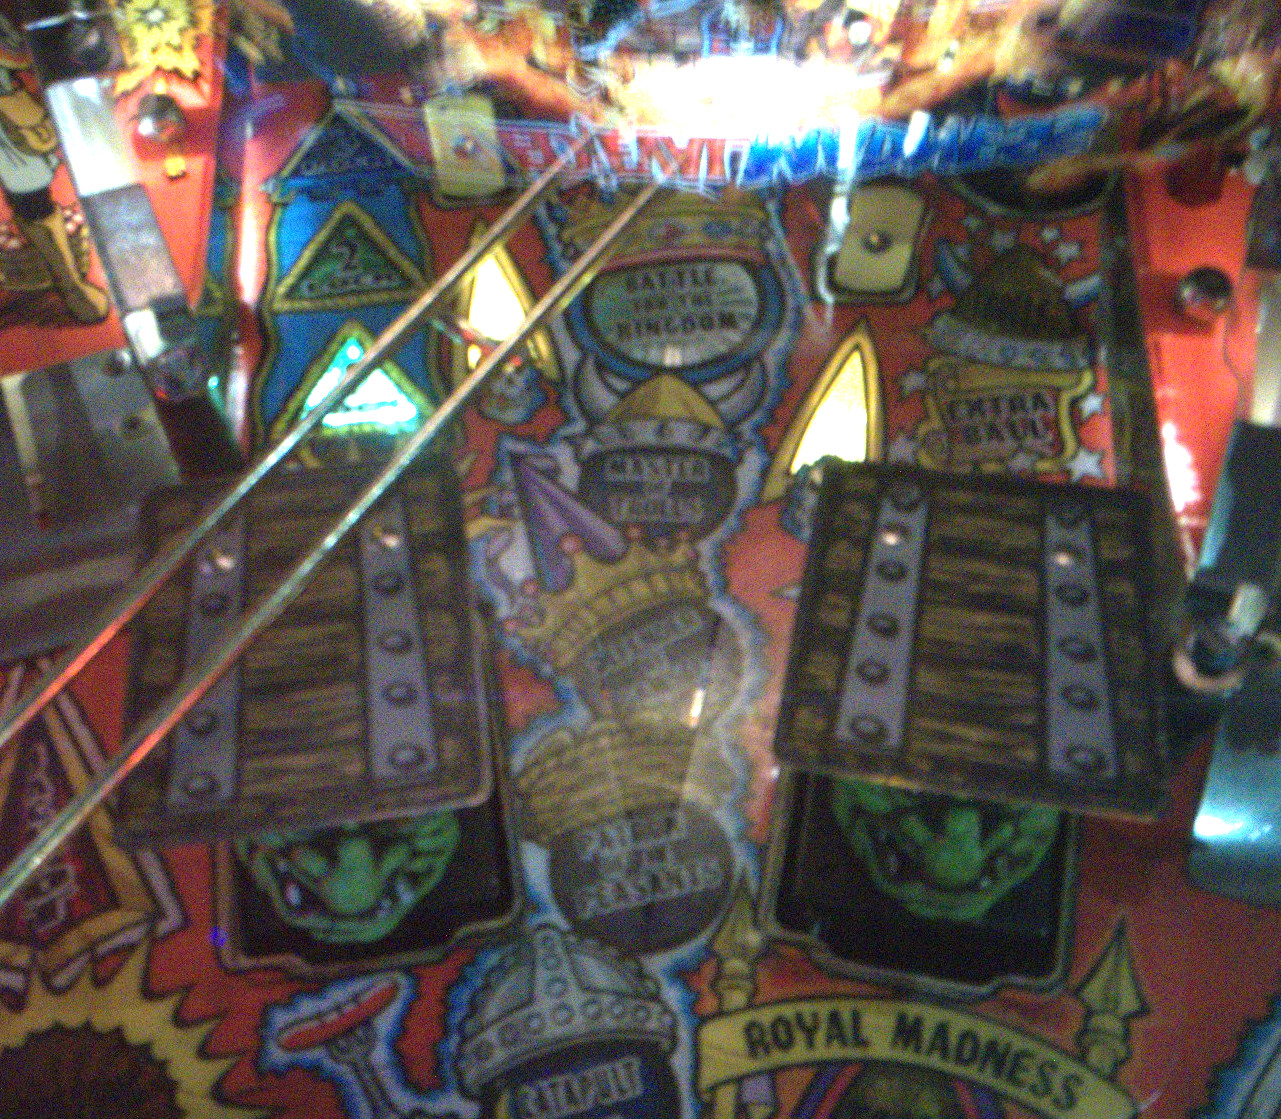
\includegraphics[height=0.4\textheight]{trolls.jpg}
\begin{itemize}
	\item Lit by yellow bumpers near castle
	\begin{itemize}
		\item Not worth shooting directly
		\item Go for castles instead
	\end{itemize}
	\item Shoot eject shot to activate
	\begin{itemize}
		\item Always best with multiball
	\end{itemize}
	\item 3 hits each to kill
	\item Requires a solid shot (face works best)
\end{itemize}
\end{frame}

\begin{frame}{Feature: Trolls (cont.)}
\begin{itemize}
	\item Left flipper to right troll, right flipper to left troll
	\item Left to left and right to right possible but circumstantial
	\item Trouble beating in multiball?  Go for them in solo play, be prepared to drain
	\item Troll bombs
	\begin{itemize}
		\item Listen for the thunder sound
		\item Launch ball button to damage troll
		\item Tip: Use as finisher
	\end{itemize}
\end{itemize}
\end{frame}

\begin{frame}{Feature: Catapult Slam}
\begin{columns}
\begin{column}{0.6\textwidth}
	\begin{itemize}
		\item Use both flippers to launch five items of various points
		\item Items cycle in left to right order
		\item Makes a noise on change
		\item Count number of noises, time based on noise count
		\item Hold to launch first item
	\end{itemize}
\end{column}
\begin{column}{0.4\textwidth}
	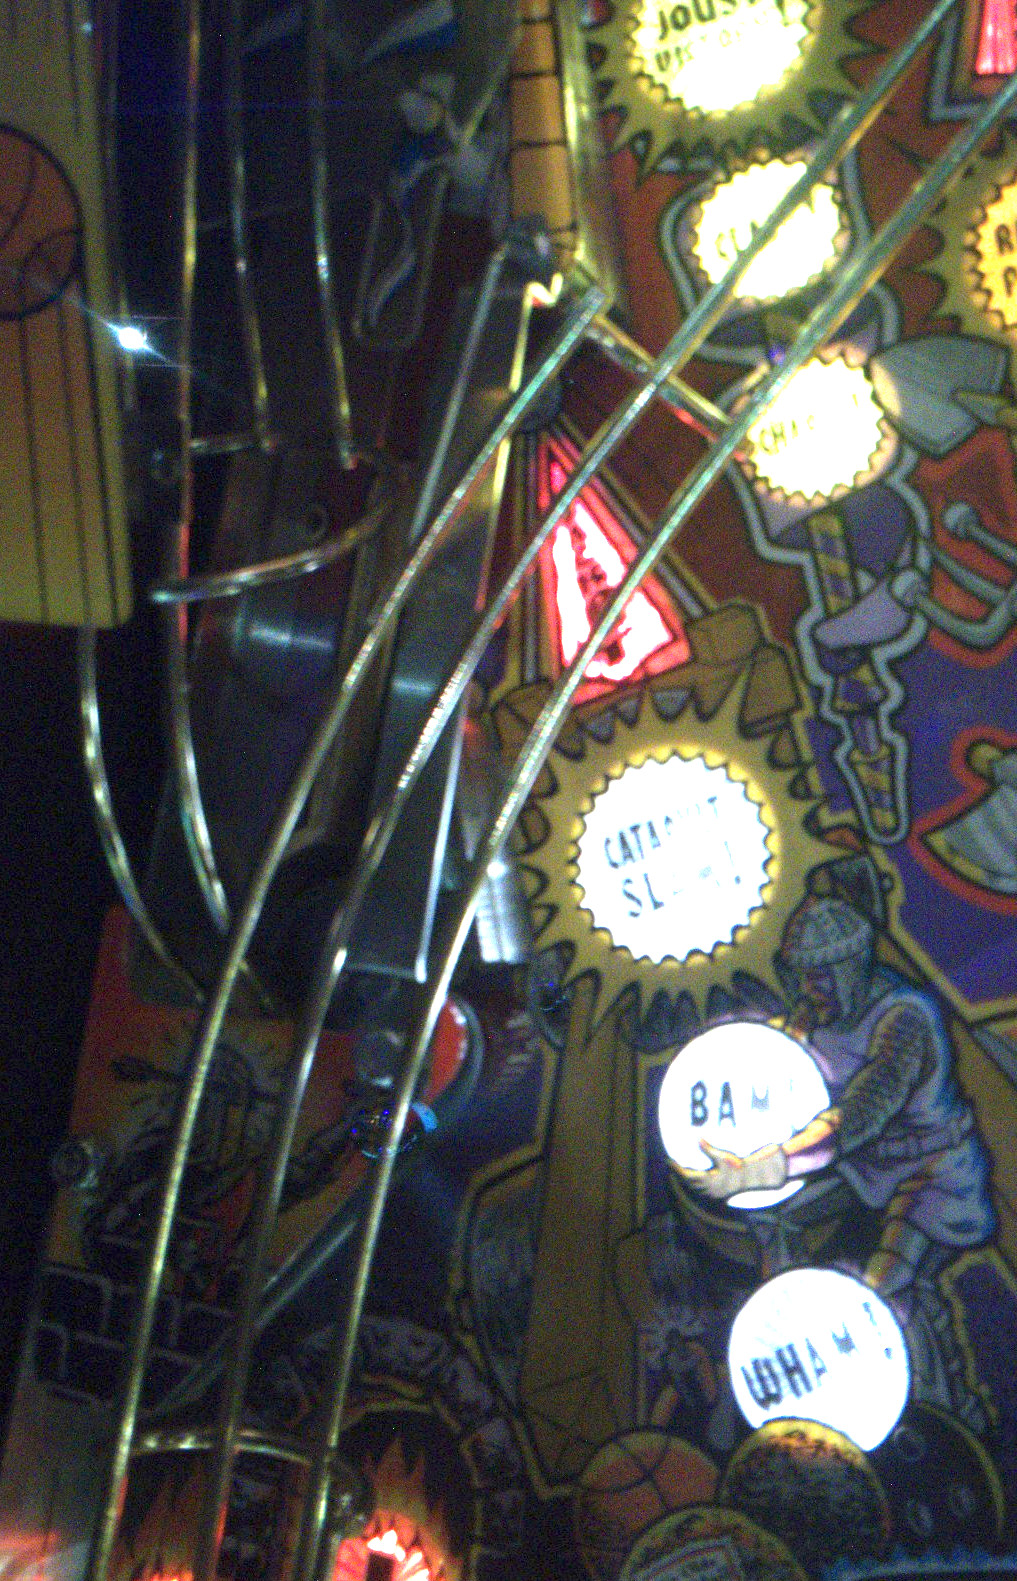
\includegraphics[width=\textwidth]{catapult.jpg}
\end{column}
\end{columns}
\end{frame}

% TODO: Picture of "ROYAL MADNESS" on display
\begin{frame}{Feature: Royal Madness}
\begin{itemize}
	\item Shoot all lanes twice and hit each troll for Extra Ball
	\item 20 second timer
	\item First shot completes lane, second shot a jackpot (1,750,000)
	\item Complete first shot on each lane to essentially double progress
	\item Troll shots ``easy'', save to prevent timeout
	\item Difficult mode to beat, very worth it
\end{itemize}
\end{frame}

\begin{frame}{Tips and Tricks}
\begin{itemize}
	\item From castle and right eject, trap ball on inner edge of flipper
	\item Impossible to trap from inner lane
	\begin{itemize}
		\item low speed: shoot to target on other side
		\item medium speed: Tip pass, castle shot
		\item high speed: Tip pass, trap on other side
	\end{itemize}
	\item Castle gate from trapped right flipper is dicey
	\begin{itemize}
		\item Lock shot or peasants instead
	\end{itemize}
	\item Castle multiball lock shot
	\begin{itemize}
		\item Very difficult shot
		\item Pass from left flipper to right eject
		\item Trap with right flipper
		\item Make lock shot
	\end{itemize}
\end{itemize}
\end{frame}

\begin{frame}{Tips and Tricks (cont.)}
\begin{itemize}
	\item Multiball madness
	\begin{itemize}
		\item Focus on trolls until ``Master of Trolls''
		\item Three+ balls: control basically impossible
		\item Two balls: Lock shot then damsel shot, trap and loop
	\end{itemize}
	\item Gutters are evil
	\begin{itemize}
		\item Horizontal momentum will drain
		\item Designed to bounce into outer lane
		\item Avoid bumpers to avoid gutters
	\end{itemize}
	\item Trouble making a shot?
	\begin{itemize}
		\item Sacrifice some games to focus on it
		\item Think long-term
		\item Only need to beat Battle for the Kingdom once!
	\end{itemize}
	\item Madness lit?  Start lighting the others
	\item Trolls lit?  Start lighting madnesses
	\item Avoid Merlin's Magic when drawbridge up
	\item First free replay?  Insert 1 credit to reset value
\end{itemize}
\end{frame}

\begin{frame}{Tier 4: Battle for the Kingdom}
\begin{columns}
\begin{column}{0.8\textwidth}
	\begin{itemize}
		\item Criteria (all center blue lights lit):
		\begin{itemize}
			\item 6 castles destroyed
			\item 10 trolls killed
			\item 3 peasant revolts, 3 damsel saves, 3 joust victories, 3 catapult slams
		\end{itemize}
		\item Shoot into castle to start
		\item 4 ball multiball
		\item Infinite time in multiball, 10 second timer in solo play
		\item Shoot each lane and lock shot for Battle Jackpot (2,500,000)
		\begin{itemize}
			\item Joust lanes are separate!
		\end{itemize}
		\item Trolls appear, invincible without troll bomb
		\item 7 gate shots (5,000,000)
		\item 1 castle shot (50,000,000)
	\end{itemize}
\end{column}
\begin{column}{0.2\textwidth}
	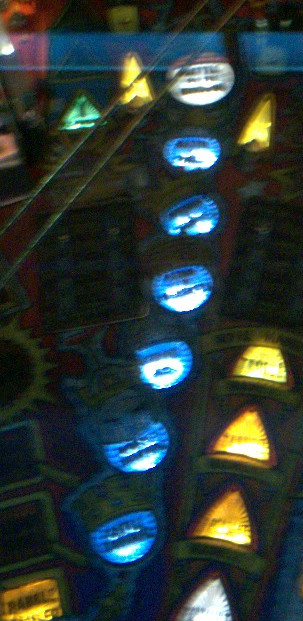
\includegraphics[width=\textwidth]{battle_for_the_kingdom.jpg}
\end{column}
\end{columns}
\end{frame}

\begin{frame}{Tier 4: Battle for the Kingdom (cont.)}
\centering 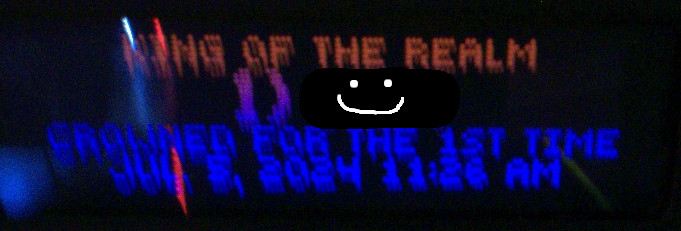
\includegraphics[width=\textwidth]{king_of_the_realm.jpg}
\begin{itemize}
	\item King of the Realm!
	\item \small lol the date is off 9 months
\end{itemize}
\end{frame}

\section{Auxiliary info}
% TODO: The "Hurry up" display would be good to have here.
\begin{frame}{Feature: Hurry ups}
\begin{columns}
\begin{column}{0.8\textwidth}
\begin{itemize}
	\item Activation
	\begin{itemize}
		\item Super skill shot
		\item Qualify madness without qualifying multiball madness
	\end{itemize}
	\item 1,000,000 points, decreases over time
	\begin{itemize}
		\item 3,000,000 points if second activated during first
		\item 5,500,000 \ldots
	\end{itemize}
	\item Shoot castle to claim
	\begin{itemize}
		\item Safest when drawbridge up\ldots
		\item Not that you have much of a choice
	\end{itemize}
	\item Claim 10 to light extra ball
	\begin{itemize}
		\item Never done this\ldots
	\end{itemize}
\end{itemize}
\end{column}
\begin{column}{0.2\textwidth}
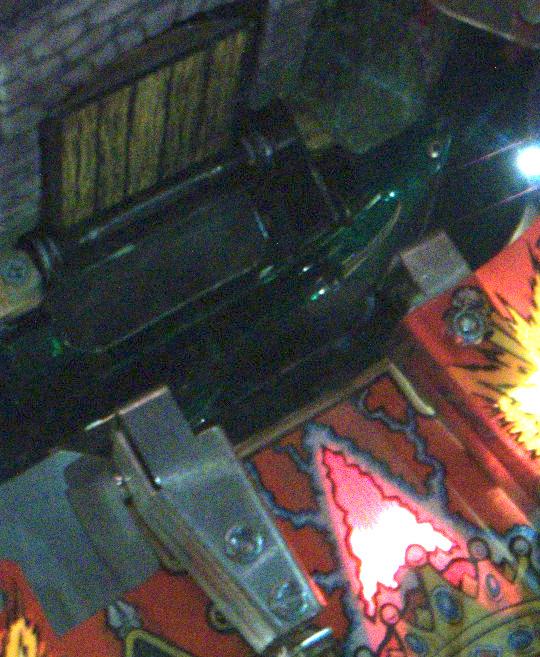
\includegraphics[width=\textwidth]{hurry_up.jpg}
\end{column}
\end{columns}
\end{frame}

% TODO: Picture of "Save the Children" gameplay
\begin{frame}{Save the children}
\begin{itemize}
	\item Light ``FIRE'' 8 times
	\item Flippers rotate lights
	\item Eject shot to activate?
	\item Video mode
	\item It's so ghetto lol
	\item Use flipper to move character; striking automatic?
	\item 4,200,000 reward on success
	\item Never done it\ldots
\end{itemize}
\end{frame}

% TODO: Picture of Barnyard multiball
\begin{frame}{Barnyard Multiball}
\begin{itemize}
	\item Catapult slam launches an item
	\item Launch one of each item
	\item 4 ball multiball
	\item All lanes jackpots
	\item Hit pops to increase jackpots
	\item Game makes silly animal noises
\end{itemize}
\end{frame}

\begin{frame}{Merlin's Magic stars}
\begin{columns}
\begin{column}{0.8\textwidth}
\begin{itemize}
	\item Hitting somehow activates Merlin's Magic
	\item I've never once aimed for them
	\item Just ignore, be glad if you get them
\end{itemize}
\end{column}
\begin{column}{0.2\textwidth}
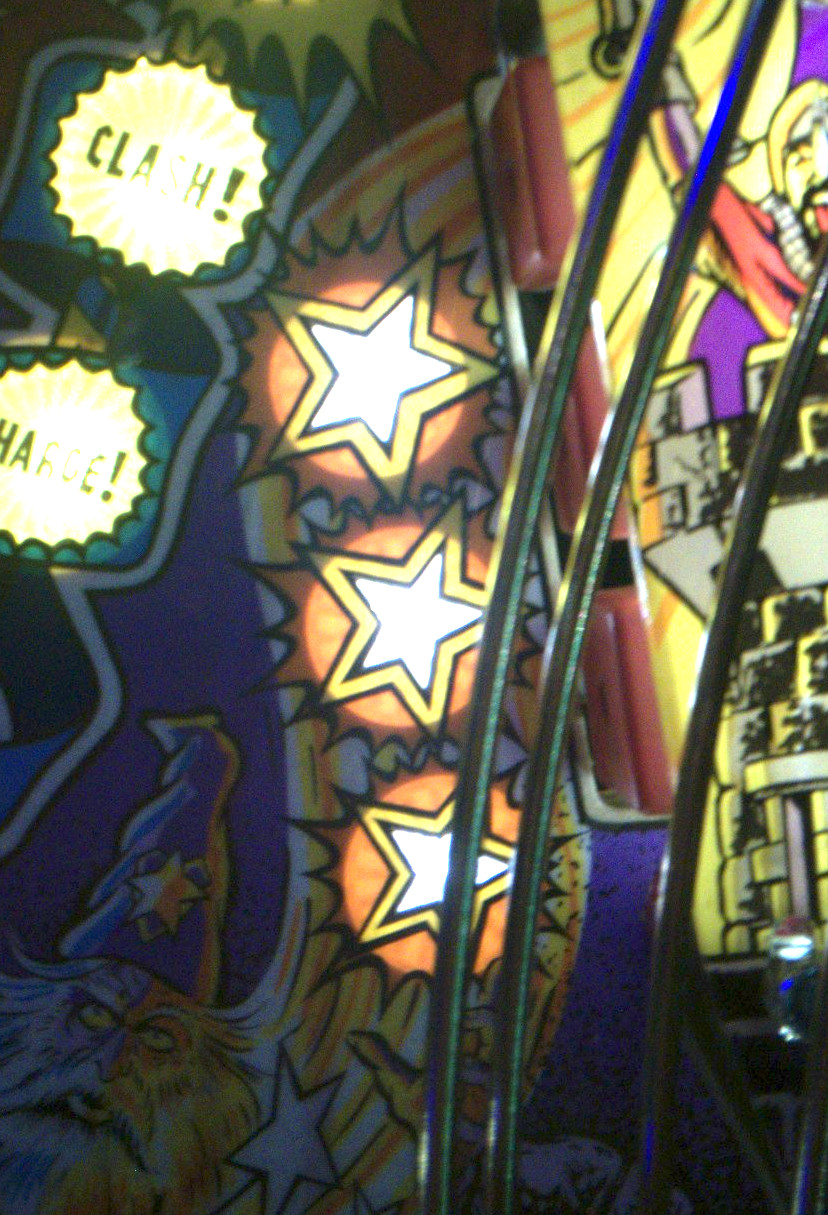
\includegraphics[width=\textwidth]{merlins_magic_stars.jpg}
\end{column}
\end{columns}
\end{frame}

\section{End}
\begin{frame}{End}
\centering 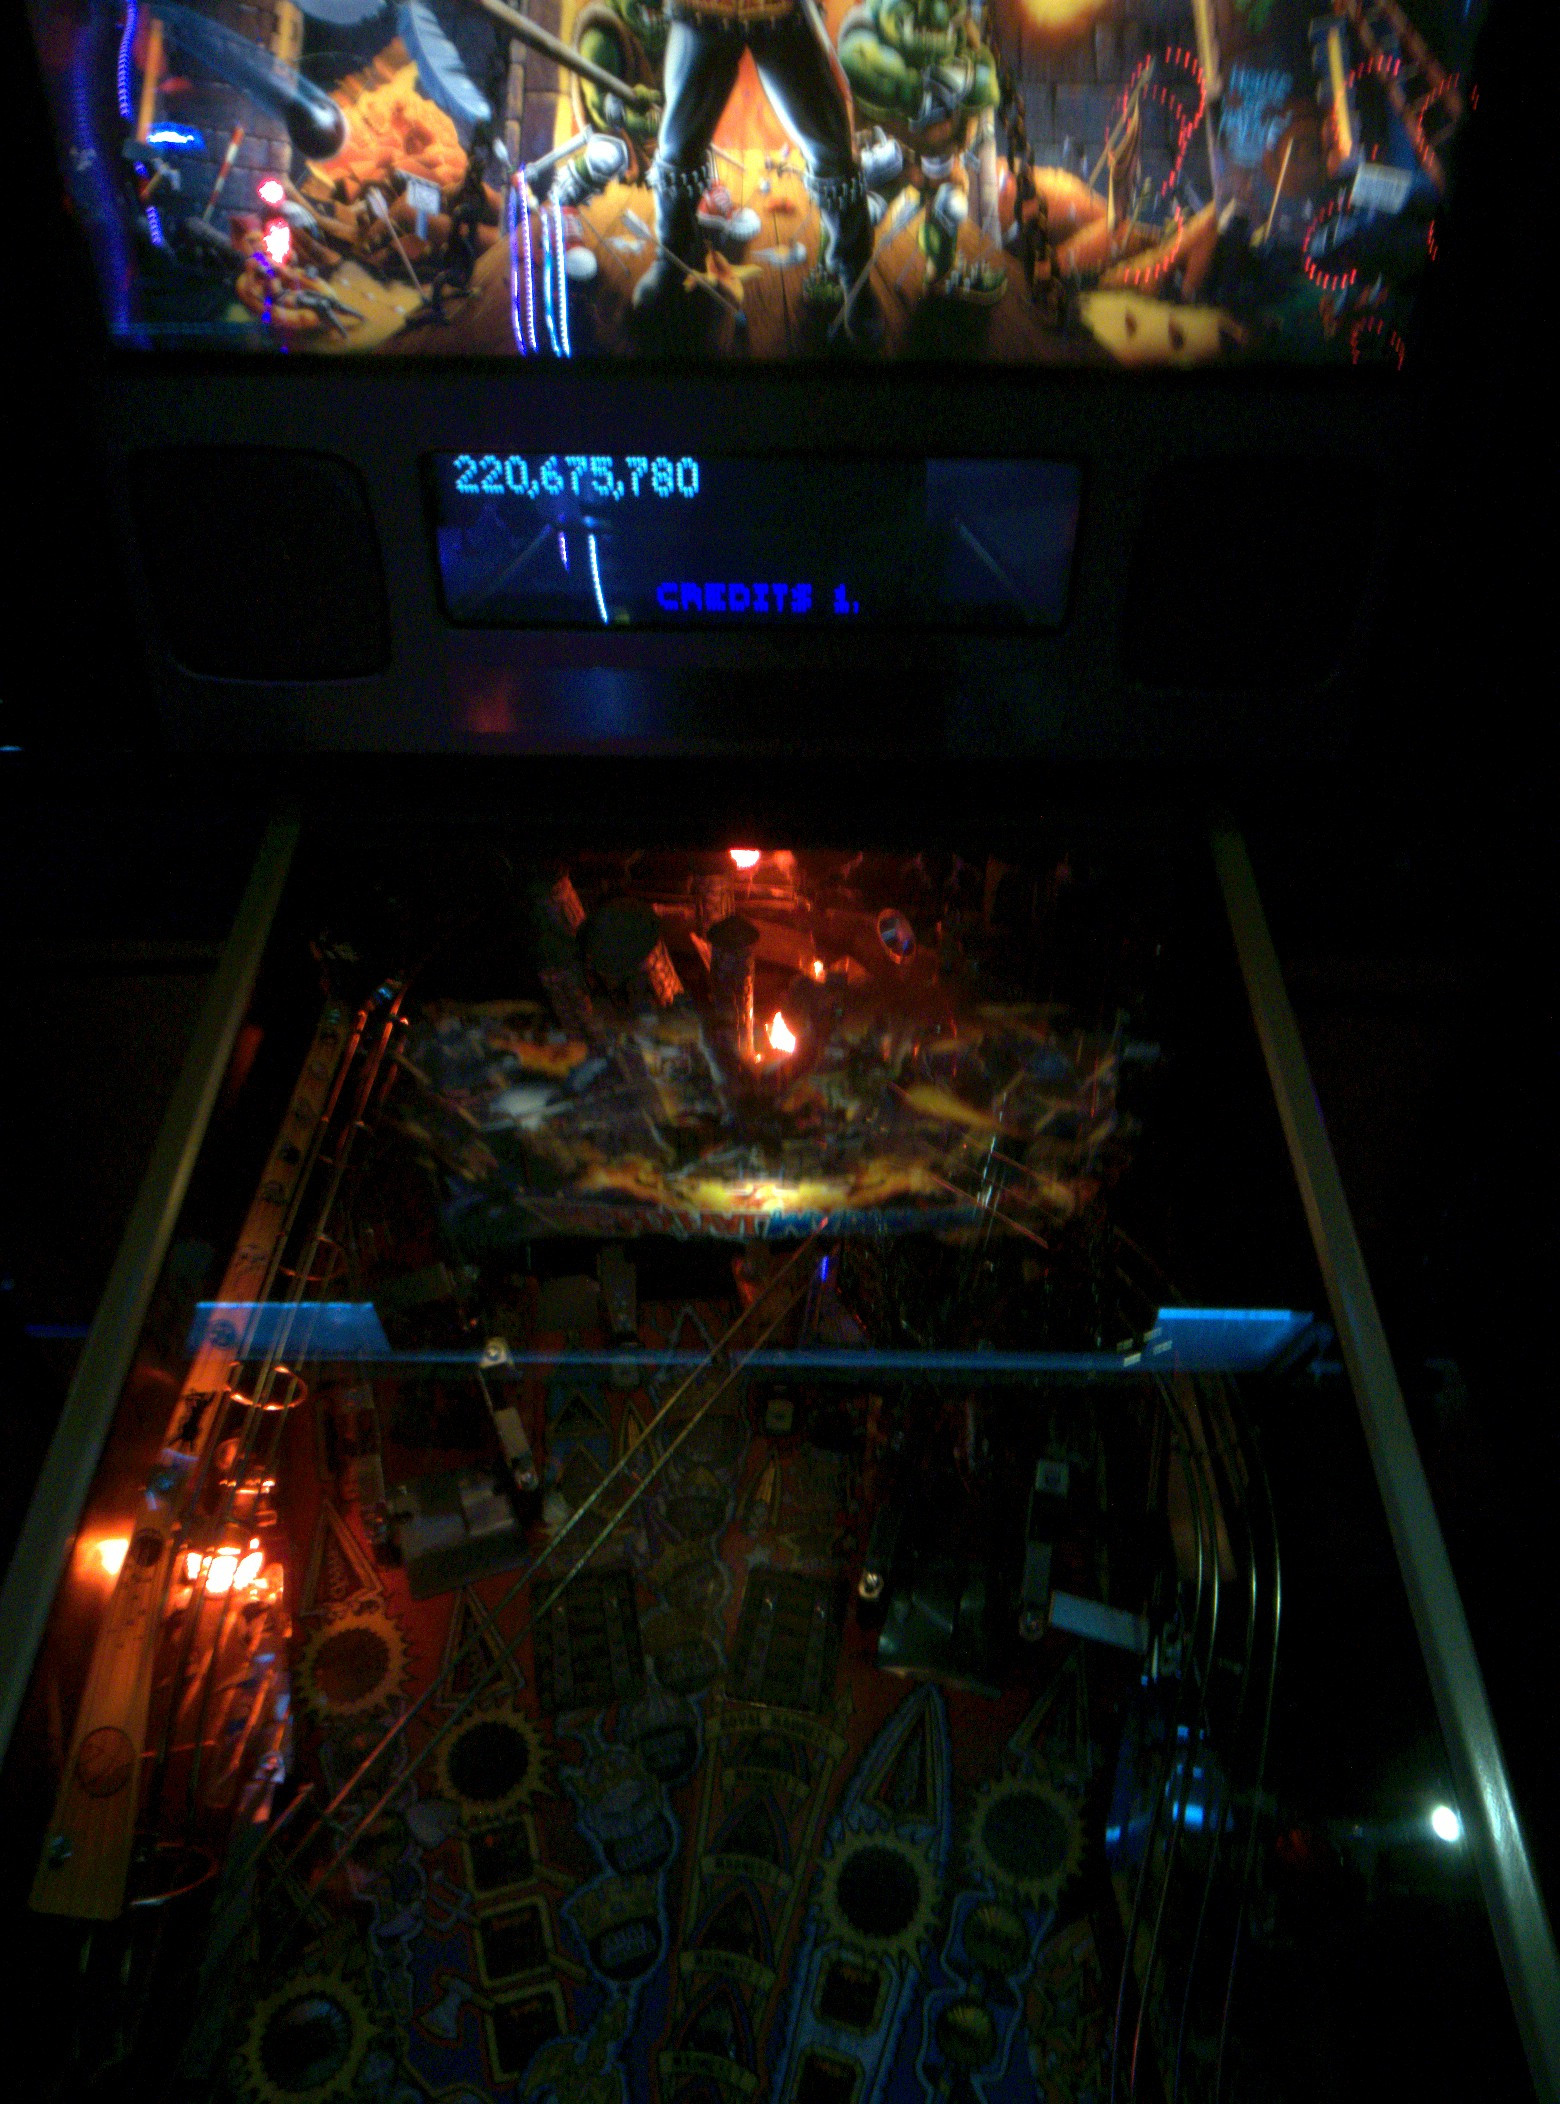
\includegraphics[height=0.8\textheight]{high_score.jpg}
\end{frame}

\end{document}
